
%-------------------------------------------------------------------------%
\section{Masses of stop particles}
Mass eigenstates of the squarks and sleptons of the MSSM can be obtained by diagonalizing three $6\times6$ (from the up- and down-type squarks and charged sleptons) and one $3\times3$ matrices (from sneutrinos) of which most are negligible due to their small mixing angles \cite{martin1997supersymmetry}. For the stops, in particular, the mass eigenstates are given by the matrices

\begin{align}
    \begin{pmatrix} \Tilde{t}_1 \\ \Tilde{t}_2 \end{pmatrix} = 
    \begin{pmatrix} \cos\theta_\Tilde{t} & -\sin\theta^*_\Tilde{t} \\ \sin\theta_\Tilde{t} & \cos\theta^*__\Tilde{t} \end{pmatrix}
    \begin{pmatrix} \Tilde{t}_L \\ \Tilde{t}_R \end{pmatrix}
    \label{eq:stopMass}
\end{align}
where $ \theta_\Tilde{t} $ is the stop mixing angle in the range $ 0 \leq {\theta_\Tilde{t}} \leq \pi $ satisfying $ |\cos\theta_{\Tilde{t}}|^2 + |\sin\theta_{\Tilde{t}}|^2 = 1 $. \\

The mass splitting of the two stops $ \tilde{t}_1 $ and $ \tilde{t}_2 $ arise from the squared-mass matrix for stops, where the off-diagonal elements involves a large top-quark Yukawa coupling ($y_t$ term) that induces such a phenomena \cite{kraml2016scalar}. Diagonalizing gives the $\Tilde{t}_L$ and $\Tilde{t}_R$ components on the right-hand side of Equation (\ref{eq:stopMass}). \\

Due to many reasons out of the scope of this review, various models predict that $\Tilde{t}_1$ is the lightest of all squarks, predominantly theorized to be $\Tilde{t}_R$ which is the right-handed stops \cite{martin1997supersymmetry}. Although there has been no success in the direct detection, therefore, a properly theorized mass, experimental efforts have been made to set constraints for the stop mass \cite{kraml2016scalar, aad2014search, abdughani2018probing, sirunyan2018search, yoshihara2017search}.

%-------------------------------------------------------------------------%
\section{Possible decay channels of the top squarks} \label{sec:stopDecay}
A well-summarized discussion about the possible backgrounds in stop production is presented in \cite{plehn2010stop}, where there are four possible modes suggested: top-pair, QCD, W+jets, and Z+jets. Note that \textit{jets} are some cluster of hadronized quarks or gluons produced in a decay since they cannot exist freely. They are used for analysis since they are well-defined, easily-to-measure/calculate and have a close correspondence to the final state of interest \cite{seymour1996jets}. \\

Quoted as ``dangerous", the top-pair production, especially the semi-leptonic top decays that we consider in this section, overwhelm the stop signals even after top-tagging (jets identified to have originated from top-decays) and signal selections made \cite{plehn2010stop}. The QCD background is said to be an``insurmountable" background at the LHC. However, it can be suppressed until below that of the $t\Bar{t}$ background by applying treatments such as ``fake" missing energy and $b$-mistagging (jets misclassified to have originated from b-quarks) and two top-tagging \cite{plehn2010stop}. The W+jets case is easier to deal with due to the apparent missing energies created from the four hard jets (plus others) that only marginally exceed that of the signal \cite{plehn2010stop}. These are dealt with basic cuts and two top-tagging \cite{plehn2010stop}. Finally, the Z+jets case can be deemed as irrelevant simply due to its significantly smaller rate \cite{plehn2010stop}. Of course, background derived from other processes will be produced in LHC experiments, however, the signatures will be different from how it originates, thus allowing the search to be narrowed down to identical processes in background and signal. From these, it is evident that the most interesting and pressing background decay to study is the semi-leptonic final state of the top quark decay. \\

Just like the SM particles and their decay dictated by known symmetries and conservation laws, the decay of stops is dictated by the parameters and kinematics suggested by MSSM. The mass of stops would significantly affect the decay modes. \\

A heavy enough stop at the order of the sum of the top quark mass and neutralino mass ($m_t+m_{\Tilde{\chi}_1^0}$)(or charginos) would undergo a two-body decay into top quarks with neutralinos: $\Tilde{t}_1\rightarrow t\Tilde{\chi}_1^0$ (or bottom quarks with charginos: $\Tilde{t}_1\rightarrow b\Tilde{\chi}_1^+$) \cite{boehm2000decays}. A lighter stop that is above the sum of the bottom quark mass, W-boson mass and neutralino mass ($m_b + m_W + m_{\Tilde{\chi}_1^0}$) would imply a three-body decay $\Tilde{t}_1\rightarrow b W \Tilde{\chi}_1^0$. Four-body decays into a combination of bottom quarks, neutralinos and SM fermions, may also be possible: $\Tilde{t}_1\rightarrow b\Tilde{\chi}_1^0 f \Bar{f}'$ \cite{boehm2000decays}. However, the four-body decay is only relevant when the two- and three-body decays are kinematically forbidden i.e. on-shell decays aren't allowed. This would also allow a flavor-suppressed decay to a charm quark: $\Tilde{t}_1\rightarrow c\Tilde{\chi}_1^0$ \cite{aad2014search}, where both this decay and the four-body decay can be very slow such that $\Tilde{t}_1$ is quasi-stable \cite{martin1997supersymmetry}. \\

An important assumption made in these decays is that $m_{\Tilde{t}_1} > m_{\Tilde{\chi}_1^0} $ so that the neutralinos remain the lightest (LSP). Additional decays become apparent when sparticles other than $\Tilde{\chi}_1^0 $ are lighter than the stop, such as the charginos $\Tilde{\chi}_1^{\pm}$.
A diagram from \cite{aad2014search} is shown in Figure \ref{fig:decayMode}, that represent the above statements under the assumption that $\Tilde{t}_1 $ and $ \Tilde{\chi}_1^0 $ are both the lightest sparticles, which could very well not be true since there is no experimental evidence to disprove nor prove as such. \\


\begin{figure}[htbp]
    \centering
    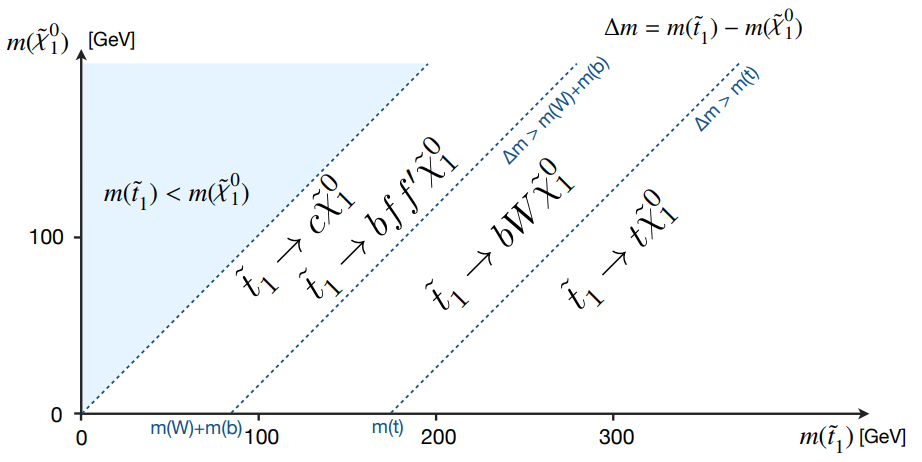
\includegraphics[width=15cm, height= 7.5cm]{decaymodes.png}
    \caption{Possible decay modes for stops within the mass-parameter-space of $\Tilde{t}_1 $ and $ \Tilde{\chi}_1^0 $ \cite{aad2014search}.}
    \label{fig:decayMode}
\end{figure}

\begin{figure}[htbp]
    \centering
    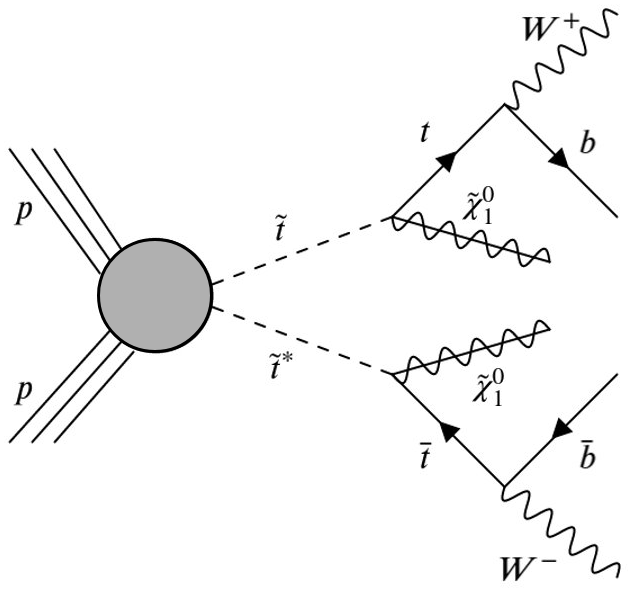
\includegraphics[width=9cm, height= 7.5cm]{stops_true.png}
    \caption{Decay chain of the signal of interest $\Tilde{t}_1 \rightarrow t\Tilde{\chi}_1^0 $.}
    \label{fig:decayInterest}
\end{figure}

For the purpose of this project, our desired background events is the process given by Equation (\ref{eq:background}) and the desired signal events given by Equation (\ref{eq:signal}). \\

\begin{equation}
 pp \rightarrow t \Bar{t} \rightarrow b\Bar{b}jjl\cancel{\it{E}}_{T},
 \label{eq:background}
\end{equation}
\begin{equation}
  pp \rightarrow \Tilde{t}\Tilde{t^*} \rightarrow t \Bar{t} \Tilde{\chi^0_1}\Tilde{\chi^0_1} \rightarrow b\Bar{b}jjl\cancel{\it{E}}_{T},
  \label{eq:signal}
\end{equation}

%-------------------------------------------------------------------------%
\section{Mass parameters for the top squarks and neutralinos}
Experiments overtime, at hte Large Hadron Collider, have set limits on the stop mass and neutralino mass. This is visually presented as an exclusion curve, such as those seen in Figure \ref{fig:limits} \cite{cms2019search}. In this particular figure, it is presented that the expected limit (in red) to the process $pp \rightarrow \tilde{t}\tilde{t}^* \rightarrow t\tilde{\chi}_1^0$ falls under that of the observed limit (in black) when both masses are high i.e. $m_{\tilde{\chi}_1^0}\approx \frac{1}{2}m_{\tilde{t}}$. It is also shown that the observed limit falls under the expected limit by a small margin when $m_{\tilde{\chi}_1^0}\ll m_{\tilde{t}}$. \\

\begin{figure}[htbp]
    \centering
    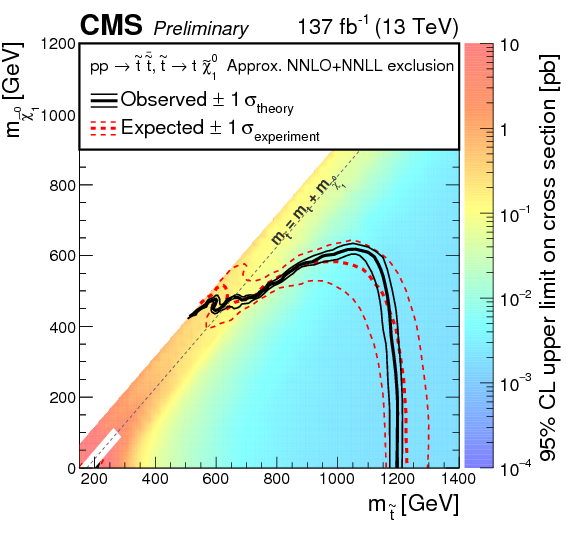
\includegraphics[width=12cm, height= 12cm]{stop_limits.png}
    \caption{The latest cross-section limit for the top squark presented in 
    \cite{cms2019search}}
    \label{fig:limits}
\end{figure}

The path sitting around $ m_{\tilde{t}} \approx 1.2$ TeV is an interesting path to follow, and observe how the algorithms presented in Section \ref{sec:method} performs. In addition, Thomas Roxlo and Matthew Reece from Harvard University \cite{roxlo2018opening} have explored the performance of their neural networks discriminating stop production to top production, albeit in a dilepton final state within the $\tilde{t} \rightarrow t \tilde{\chi}_1^0$ decay. Their choice of mass parameters are the parameters our fourth benchmark explores: $m_{\tilde{t}} =750$ GeV and $m_{\tilde{\chi}_1^0} = 1$ GeV, well within the exclusion limit in Figure \ref{fig:limits}. Table \ref{tab:benchmarks} shows a summary of mass parameters chosen to explore. 

\begin{table}[htbp]
    \centering
    \begin{tabular}{c|c|c|c} 
    \toprule
    Benchmark No. & Position & $\Tilde{t}$ Mass (TeV) & $\Tilde{\chi}_1^0$ Mass (GeV) \\
    \midrule
    \rowcolor{gray!6} 1 & Outside & $ 1.2 $ & $ 600 $ \\
    2 & Outside & $ 1.225 $ & $ 400 $ \\
    \rowcolor{gray!6} 3 & Outside & $ 1.25 $ & $ 100 $ \\
    4 & Inside & $ 0.75 $ & $ 1 $\\
    \bottomrule
    \end{tabular}
    \caption{Chosen parameters for building classifiers} 
    \label{tab:benchmarks}
\end{table}

%-------------------------------------------------------------------------%
\section{Cut-based searches}